\section{Paketverlust erkennen}
\label{sec:Paketverlust erkennen}

\subsection{Vorgehen bei Paketverlust}

Falls ein Übertragungsmedium nicht korrekt funktioniert, ist es möglich, dass Datenpakete nicht am Ziel oder mit einer zu grossen Verspätung ankommen.
Da jedes \esp{} Paket mit einer Sequenznummer versehen ist, können diese Paketverluste erkannt und gemeldet werden.

Die \esp{} Pakete besitzen zum Schutz vor Replay-Angriffen eine Sequenznummer sowie einen bestimmten Gültigkeitsbereich (Windowsize).\\
Die Pakete können zum Beispiel durch Loadbalancing \"{u}ber unterschiedliche Pfade verschickt werden. Dadurch kann die Reihenfolge der Pakete am Ziel nicht mehr gewährleistet werden. Die zu spät ankommenden Pakete müssen daher überprüft werden, ob die Sequenznummer aktuell noch gültig ist (innerhalb des Window).

\todo{Jan: Caption bei Grafik hinzufügen}

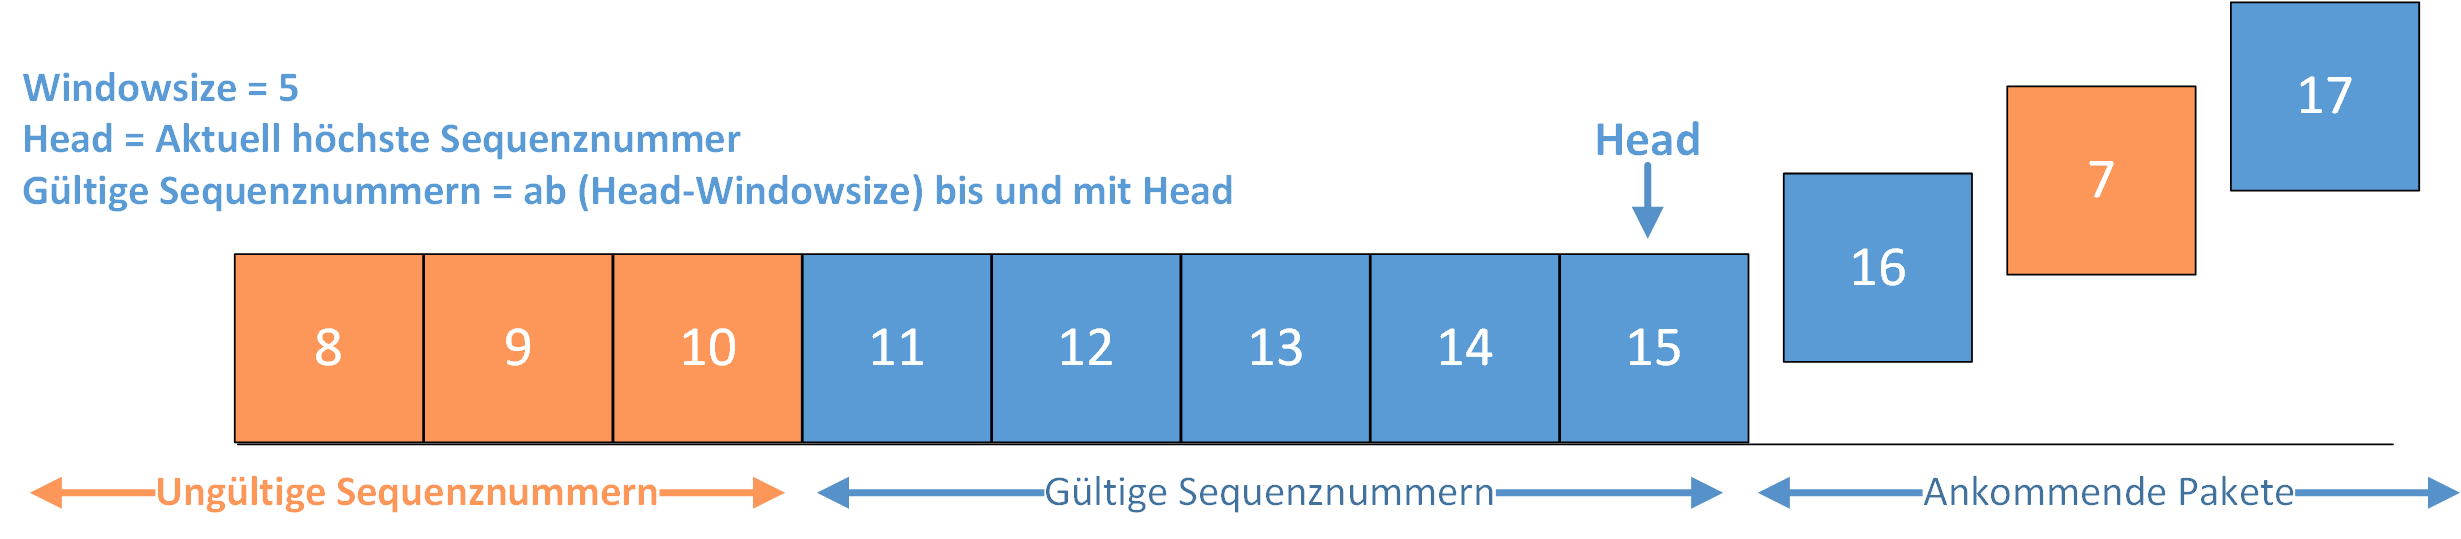
\includegraphics[width=1\textwidth]{start/img/Sequenznummern.png}

\subsection{Datenstruktur für die \esp Verbindungen}
Pro Verbindung werden separate Sequenznummern verwendet. Die verschiedenen Verbindungen werden durch eine Hashmap verwaltet. Als Key wird eine Struktur aus Source, Destination und \acs{SPI} verwendet. Als Value werden grundsätzlich zwei Listen für die Lost und MaybeLost Pakete benötigt. Zusätzlich wird noch ein Wert für den aktuellen Head gespeichert.

\todo{Jan: Caption bei Grafik hinzufügen}

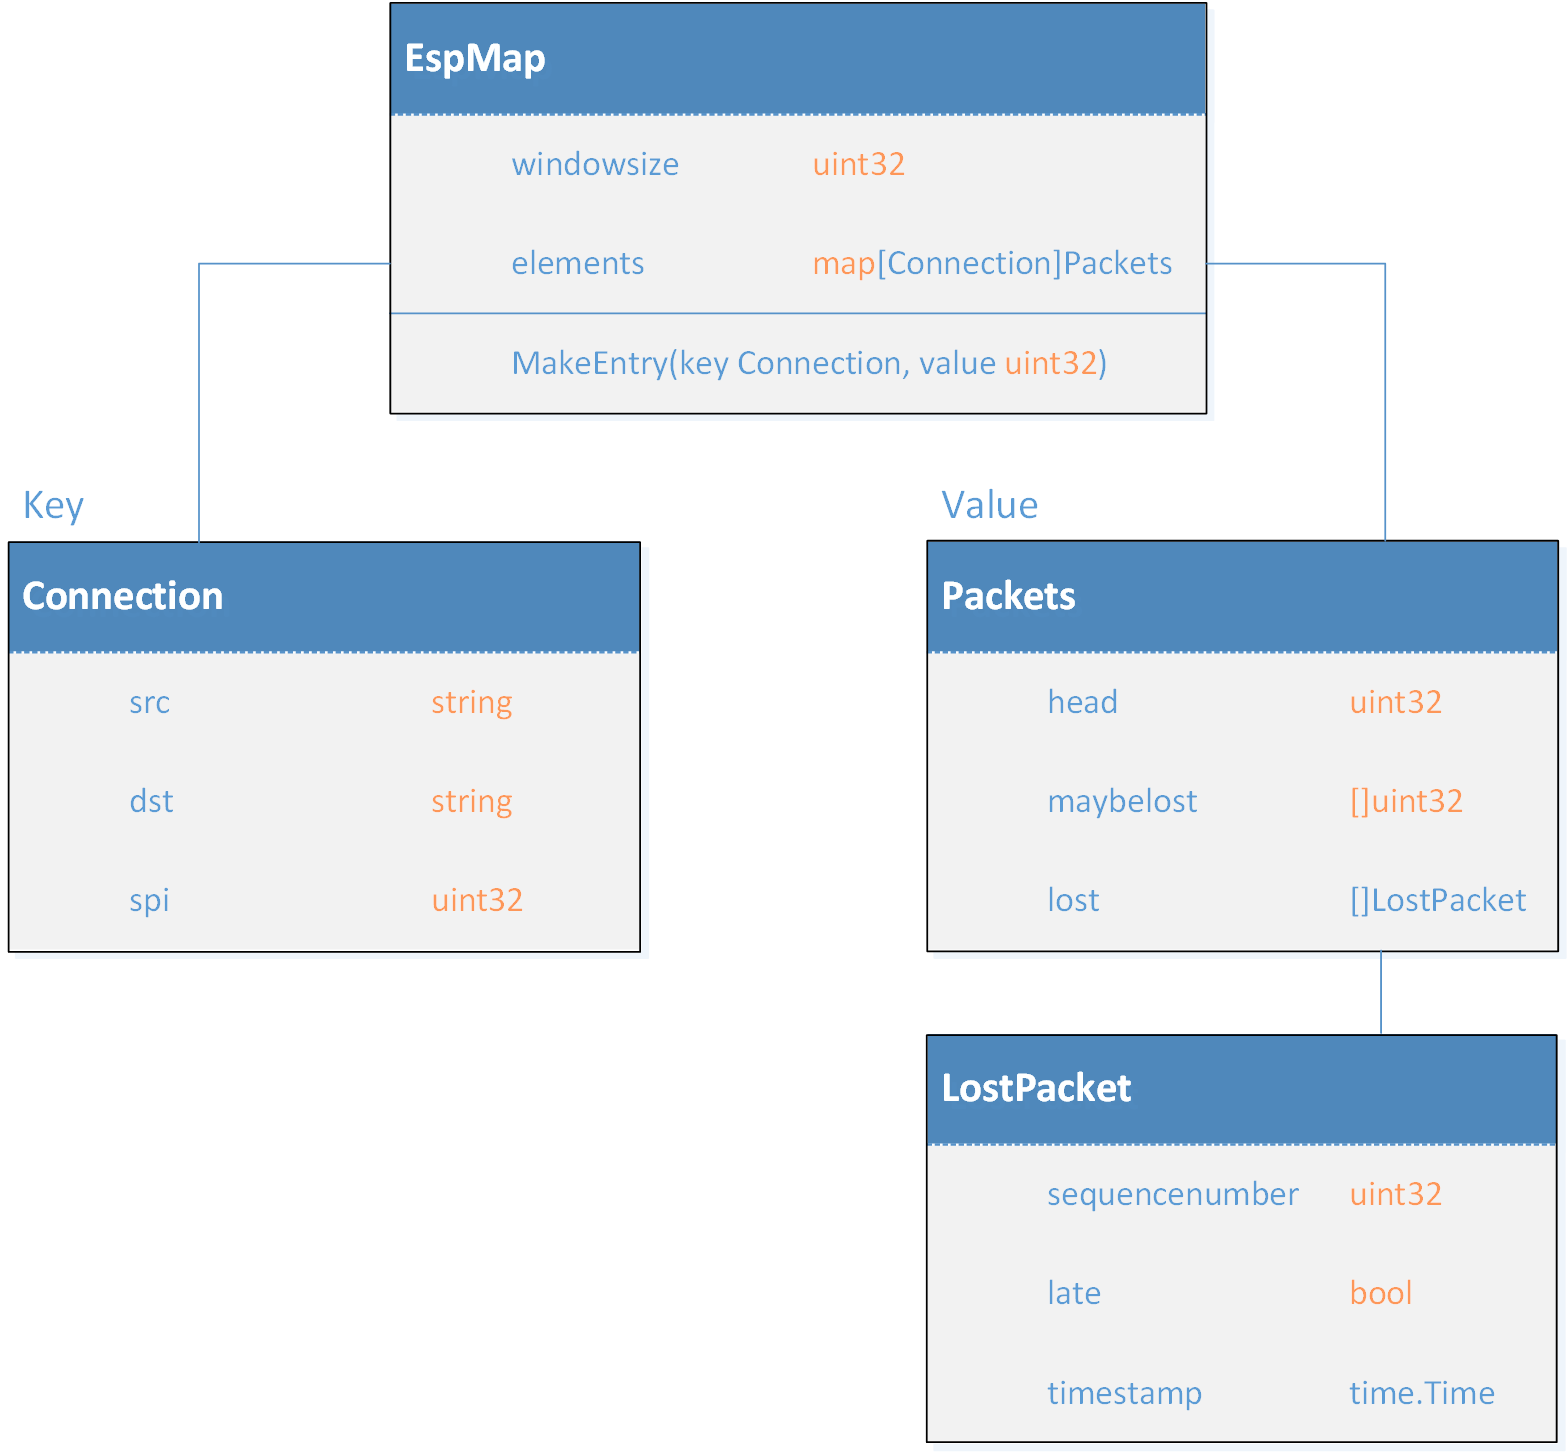
\includegraphics[width=1\textwidth]{start/img/Datenstruktur.png}

\subsection{Erkennung des Paketverlusts}
Die Paketverluste werden mit folgendem Algorithmus festgestellt.
Vereinfachte Darstellung des Algorithmus in Pseudocode:
\\
\textbf{Neues Packet Verarbeiten}
\begin{lstlisting}[language=go]
if(neuesPacket > Head){
	if(neuesPacket != Head + 1){
		Packete von Head bis neuesPacket in 
		MaybeLost speichern
	}
	Head = neuesPacket
	CheckLost()
}else{
	if(Head-WindowSize < neuesPacket){
		Packet aus MaybeLost entfernen
	}else{
		Flag fuer zu spaet angekommen setzen	
	}
}
\end{lstlisting}

\textbf{CheckLost}
\begin{lstlisting}[language=go]
for(MaybeLost){
	if(Head-WindowSize >= MaybeLostEintrag){
		Packet in Lost Speichern
		Packet aus MaybeLost entfernen
	}
}
\end{lstlisting}


\section{ Meldungsaufbau}

\noindent Die Bedingungen für das Auslösen eines Alerts können im Configfile festgelegt werden. Es können der Zeitraum und die Anzahl Pakete definiert werden. Falls innerhalb dieses definierten Zeitraums die Anzahl an verlorenen Paketen überschritten wird, wird ein Alert ausgelöst.

\noindent Der Alert besitzt folgende Form:

\begin{tabular}{|p{0.5in}|p{0.7in}|p{3.0in}|} \hline 
Severity & Programm & Meldung \\ \hline 
1 & IPsecDiagTool & Too much LostPackets in Connection: (SPI: \dots ,SRC:\dots ,DST\dots ) \\ \hline 
\end{tabular}

\todo{Tabelle überschneidet sich.}

\noindent So kann gleich anhand der Meldung erkannt werden, um welche Verbindung es sich handelt und die notwendigen Schritte für eine Korrektur vorgenommen werden.

\noindent Damit es nicht zu einer Flut von Benachrichtigungen mit dem gleichen Inhalt und den gleichen Paketen kommt, wurde ein Timer von 10 Sekunden eingeführt.

\section{ Logging Package}

\noindent Das Logging wurde in einem separaten Package umgesetzt und stellt Methoden für das Logging zur Verfügung. Die Package kapselt die benötigte Funktionalität, die von \code{log/syslog} benötigt wird.

\noindent Das Package wird vor Verwendung der Logging Funktionalität durch InitLogger initialisiert. Dabei werden die Werte für Zeitfenster, Anzahl Packete und Syslogserver gesetzt. Danach können die Benachrichtigungen mit AlertLog und InfoLog erstellt werden.

\section{ Benachrichtigung mit Datei}

\noindent Gleichzeitig mit dem Syslogeintrag wird eine CSV Datei erstellt. Die Datei beinhaltet detaillierte Informationen um welche verlorenen Pakete es sich handelt und mit welchem Abstand ein Verlust detektiert wurde. Ausserdem gibt es Informationen, ob ein Paket möglicherweise zu spät eingetroffen ist (also ausserhalb des Windows für die Sequenznummern). Falls dieses Problem vermehrt eintritt, könnte ein Erhöhen der Window-Size nötig sein.

\noindent Die Datei wurde so angepasst, dass sie mit Microsoft Excel oder ähnlichen Programmen problemlos gelesen und weiter verarbeitet werden kann.

\noindent Beispiel einer Datei

\begin{tabular}{|p{0.9in}|p{1.7in}|p{0.8in}|} \hline 
\multicolumn{2}{|p{1in}|}{SPI:12345 SRC: 192.168.0.1 DST: 192.168.0.2} &  \\ \hline 
Sequencenumber & Timestamp & ReceivedLater \\ \hline 
2 & Monday, 04-May-15 11:53:42 CEST & false \\ \hline 
3 & Monday, 04-May-15 11:53:42 CEST & true \\ \hline 
4 & Monday, 04-May-15 11:53:42 CEST & false \\ \hline 
5 & Monday, 04-May-15 11:53:42 CEST & false \\ \hline 
\end{tabular}

\todo{Tabelle mit Caption versehen und Überschneiden beheben.}